
\documentclass[aspectratio=1610, 13pt]{beamer}
%\usepackage{ctex}
%\usepackage{CJKutf8}

%\setCJKmainfont[ItalicFont=Noto Sans CJK SC Bold, BoldFont=Noto Serif CJK SC Black]{Noto Serif CJK SC}

\usepackage{xcolor}
\usepackage{multicol}
\usepackage{mathtools,array}
\usepackage[T1]{fontenc}
\usepackage{zi4}
\usepackage[font={scriptsize,bf}]{caption}
% \usepackage{subcaption}
\usepackage{graphics}
\usepackage{tikz}
\usepackage{fontawesome5}
\usepackage{mathpartir}

\newcommand{\naturals}{\mathbb{N}}
\newcommand{\reals}{\mathbb{R}}

\newcommand{\Dist}[1]{\mathcal{D}(#1)}
\newcommand{\expectation}{\mathbb{E}}

\newcommand{\states}{S}
\newcommand{\actions}{A}
\newcommand{\observables}{O}
\newcommand{\trans}{T}
\newcommand{\obs}{Z}
\newcommand{\reward}{R}
\newcommand{\discount}{\gamma}

\newcommand{\beliefs}{\mathcal{B}}
\newcommand{\beliefUpdate}{\tau}

\newcommand{\policy}{\pi}

\newcommand{\diff}[1]{\mathop{}\!\mathrm{d}#1}
\renewcommand{\figurename}{Figure}
\renewcommand{\refname}{Reference}

\AtBeginDocument{
  \catcode`_=12
  \begingroup\lccode`~=`_
  \lowercase{\endgroup\let~}\sb
  \mathcode`_="8000
}

% \usetheme{Madrid}
% % \usetheme{default}
% \setbeamertemplate{caption}[numbered]
% \setbeamerfont{title}{size=\large}
\mode<presentation>
{
  \usetheme{Darmstadt}      % or try Darmstadt, Madrid, Warsaw, ...
  \usecolortheme{default} % or try albatross, beaver, crane, ...
  \usefonttheme[onlymath]{serif}  % or try serif, structurebold, ...
  \setbeamertemplate{navigation symbols}{}
  \setbeamertemplate{caption}[numbered]
  \setbeamertemplate{footline}[frame number] 
} 

\usepackage{listings}
\lstdefinestyle{heaplang}{
    language=C,
    basicstyle=\footnotesize\ttfamily,
    keywordstyle=\color{blue},
    commentstyle=\color{red},
    escapeinside={<@}{@>},
    morekeywords={new_chan, fork, recv, send, swap, ref}
}
\lstdefinestyle{clang}{
    language=C,
    basicstyle=\footnotesize\ttfamily,
    keywordstyle=\color{blue},
    commentstyle=\color{red},
    escapeinside={<@}{@>},
}
\lstset{style=heaplang}

\usepackage{natbib}

\newcommand{\buchi}{B\"uchi }

\definecolor{goldenpoppy}{rgb}{0.99, 0.76, 0.0}
\definecolor{goldenyellow}{rgb}{1.0, 0.87, 0.0}
\definecolor{green2}{rgb}{0.1,0.7,0.3} 
\newcommand{\gcheck}{{\color{green2}\faCheckCircle[regular] }}
\newcommand{\rcross}{{\color{red} \faTimesCircle[regular]} }
\newcommand{\rflag}{{\color{red} \faFlag}}
% \usepackage{algorithm,amsmath}
% \usepackage[noend]{algpseudocode}

\newcommand{\zlstinline}{\let\par\endgraf\lstinline}
\newcommand{\comments}[1]{{\color{red}#1}}
\title{Deciding Memory Safety for Single-Pass Heap Manipulating Programs}
\date{\today}
\author{POPL 2020\\Umang Mathur et al.}
\begin{document}
\maketitle

\begin{frame}{Problems Considered}

Automatic verification of Heap-manipulating programs:

\begin{itemize}
\item Assertion checking:  deacidable reasoning.
\item Memory safety: no access outside the allocated locations. 
\end{itemize}
\begin{center}
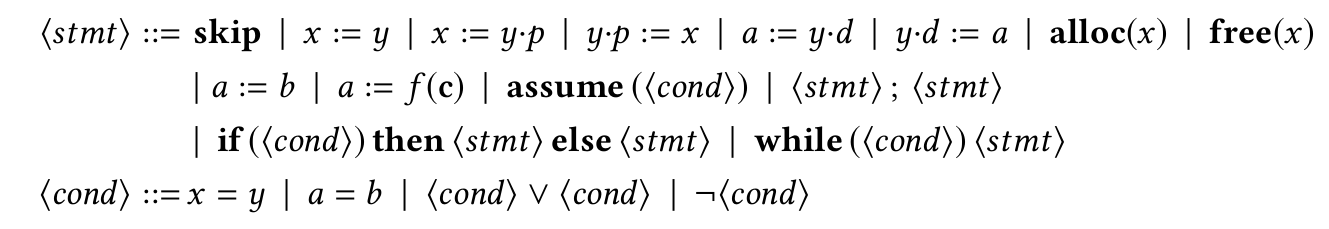
\includegraphics[scale=0.28]{program_syntax.png}
\end{center}
\end{frame}

\begin{frame}{Previous Work}

\begin{itemize}
\item [{[1]}] Umang Mathur et al. Decidable Verification of Uninterpreted Programs. POPL 2019

\textbf{Coherent Program}: Admit decidable verification.

For program without heap manipulating statements.
\end{itemize}

\end{frame}


\begin{frame}\frametitle{Contributions}
\begin{itemize}
\item Assertion checking:
\begin{itemize}
\item Coherence is not enough.

\item A Class of heap-manipulating program: alias-awareness.


\item Alias-awareness + Coherence: decidable and PSPACE-complete.

\end{itemize}
\item Memory safety:

\begin{itemize}
\item A class of heap structure.

\item Forest data-structures are alias-aware.

\item Initial forest data-structures + streaming coherence: decidable.
\end{itemize}
\end{itemize}


\end{frame}


\begin{frame}\frametitle{Uninterpreted Programs}

\begin{itemize}
\item Programs with constants, functions and predicates that are uninterpreted.
\item Signature $\Sigma = (\mathcal{C}_{\text{Data}}, \mathcal{F}_{\text{Data}\rightarrow \text{Data}}, \mathcal{R})$
\item Model $M = \langle A, \mathcal{I}\rangle$


\item Interpretations are given by the models.

\textbf{Syntax:}

\begin{center}
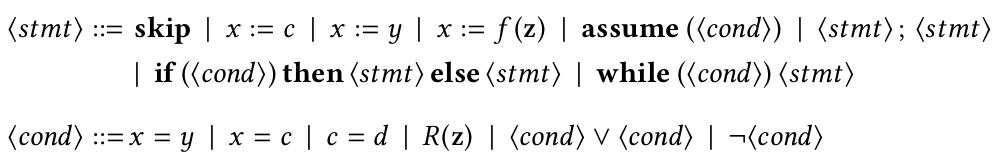
\includegraphics[scale=0.36]{syntax.png}
\end{center}
\end{itemize}
\end{frame}

\begin{frame}\frametitle{Verification Problem for Uninterpreted Programs}
\[P\models \phi\]

iff

\begin{enumerate}
\item for every model $M$, and 
\item for every execution $\rho$ feasible of $P$ under the model $M$,

$\phi$ holds in $M$ at the end of $\rho$.

\end{enumerate}

\end{frame}

\begin{frame}\frametitle{Executions and Terms}

\begin{itemize}
\item Execution: Alphabet $\Pi$ is the set of all elementary statements. The set of executions can be recursively defined by regular expression.

\item Terms: Recursively defined, variables, constants, functions..
\end{itemize}
\begin{example}
\begin{center}

\texttt{assume(x != y); \\x := f(x);\\ y := f(y);\\ x := f(x); \\y := f(y); \\assume(x = y);}
\end{center}
\end{example}

Terms symbolically represent values across different models.


\end{frame}

\begin{frame}{Coherence}

\begin{definition}[Coherence]
A Execution is coherent if
\begin{itemize}
\item Memoizing: term computed along the execution must always be stored in some variable.
\item Early assumption: making equality assumptions before forgetting superterm.
\end{itemize}

A program is coherent if all its executions are coherent.
\end{definition}

\begin{example}

\begin{center}
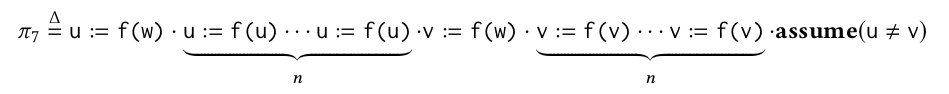
\includegraphics[scale=0.4]{coherent_exp.png}
\end{center}
\end{example}

\end{frame}

\begin{frame}\frametitle{Decidability of Verification Problem of Uninterpreted Program}
In [1] the decidability of coherent programs is proved.
\end{frame}

\begin{frame}\frametitle{Heap Manipulating Programs}
\begin{itemize}
\item Programs with constants, functions, pointers that are uninterpreted.
\item Signature $\Sigma = (\mathcal{C}_{\text{Data}}, \mathcal{C}_{\text{Loc}}, \mathcal{F}_{\text{Loc}\rightarrow \text{Data}}, \mathcal{F}_{\text{Loc}}, \mathcal{F}_{\text{Data}})$
\item Model $M = \langle U_{\text{Data}}, U_{Loc}, \mathcal{I}\rangle$


\item Interpretations are given by the models.

\textbf{Syntax:}

\begin{center}
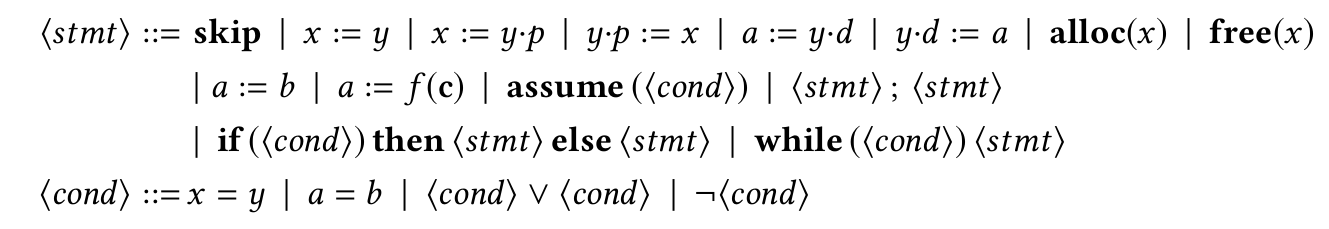
\includegraphics[scale=0.28]{program_syntax.png}
\end{center}
\end{itemize}
\end{frame}

\begin{frame}\frametitle{Example}

\begin{multicols}{2}
\begin{center}

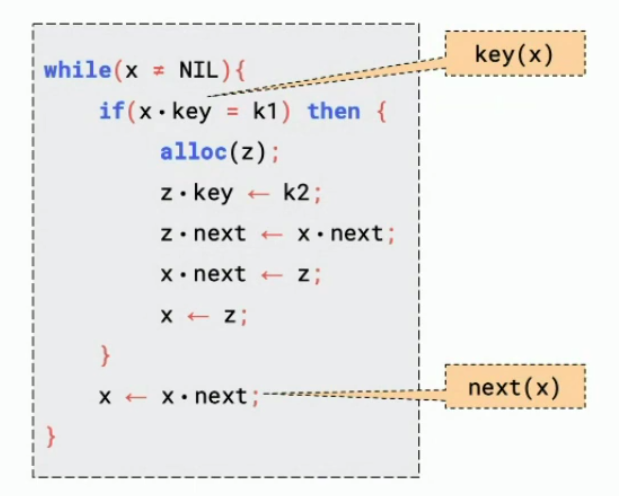
\includegraphics[scale=0.35]{hmp.png}
\end{center}
\vspace{2cm}
\begin{itemize}
\item Pointer fields are similar to uninterpreted functions + updatable.

\item Coherene and decidability?
\end{itemize}






\end{multicols}

\end{frame}

\begin{frame}\frametitle{Coherence is not enough}
\textbf{Counterexample: }
\begin{example}
\texttt{z1 := x.next;\\assume(z1 != z2);\\ y.next := z2;\\ z3 := x.next;}

\texttt{assume(z2 = z3);}
\end{example}

Consider \texttt{Term(z3)} under \texttt{x = y} and \texttt{x != y}.


The result of the verification depends on the aliasing information.

\end{frame}

\begin{frame}\frametitle{Alias-awareness}
\begin{definition}[Alias-aware]
An execution $\rho$ is called alias-aware if for every prefix of $\rho$ that is of the form $\sigma \cdot x.h := u$, the aliasing relationship between $x$ and all other location variables are known.

\end{definition}


Alias-awareness + coherence: checking assertion of heap manipulating programs are decidable


\end{frame}

\begin{frame}\frametitle{Memory Safety for Heap Manipulating Programs}
\begin{center}
Alias-awareness + Coherence
\end{center}
Forest data-structure
\begin{center}
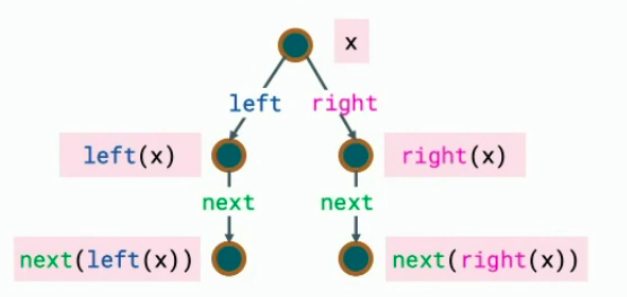
\includegraphics[scale=0.33]{forest_pic.png}
\end{center}
Intuition: Distinct traversal starting from same/different locations are distinct.




\end{frame}

\begin{frame}{Forest Data Structure}
\begin{center}
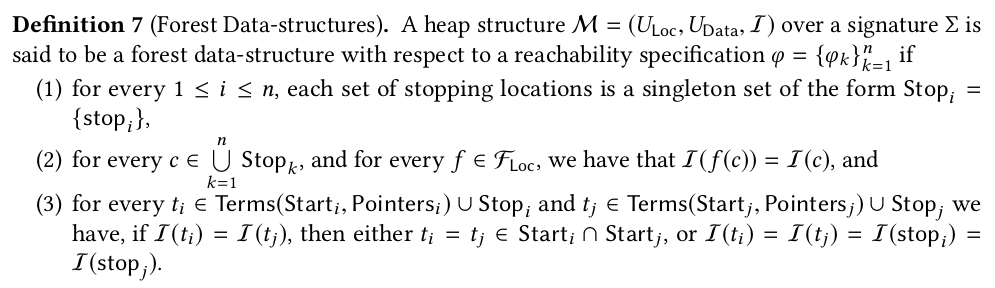
\includegraphics[scale=0.4]{forest_def.png}
\end{center}
\end{frame}

\begin{frame}\frametitle{MemSafety: Basic Idea of Decision Procedure}

\begin{itemize}
\item 
With the result in [1], we can prove execution of coherent programs are regular.
\item 
Basic Idea: construct an automaton $\mathcal{A}_{MS}$ that its languange is exactly all the coherent executions that are memory safe.

\item Check $\mathtt{Exec}(P)\subseteq L(\mathcal{A}_{MS})$.

\item which can be reduced to checking intersection of regular language.
\end{itemize}



\end{frame}

\begin{frame}\frametitle{Experimental Evaluation}

\end{frame}

\end{document}